\TOWRITE{NT/...}{Finalize}
\TOWRITE{JC}{Proofread concept and approach pass 1}
\TOWRITE{ALL}{Proofread concept and approach pass 2}

\subsection{Concept and Approach}\label{sec:concept}
\eucommentary{5-8 pages}
\eucommentary{
-- Describe and explain the overall concept underpinning the project.
Describe the main ideas, models or assumptions involved. Identify
any trans-disciplinary considerations;
-- Describe and explain the overall approach and methodology, distinguishing, as
appropriate, activities indicated in the relevant section of the work programme, e.g.
Networking Activities, Service Activities and Joint Research Activities, as detailed in
the Part E of the Specific features for Research Infrastructures of the Horizon 2020
European Research Infrastructures (including e-Infrastructures) Work Programme 2014-
2015;\\
-- Describe how the Networking Activities will foster a culture of co-operation between the
participants and other relevant stakeholders.\\
-- Describe how the Service activities will offer access to state-of-the-art infrastructures,
high quality services, and will enable users to conduct excellent research.\\
-- Describe how the Joint Research Activities will contribute to quantitative and qualitative
improvements of the services provided by the infrastructures.\\
-- As per Part E of the Work Programme, where relevant, describe how the project will
share and use existing basic operations services (e.g. authorisation and accounting
systems, service registry, etc.) with other e-infrastructure providers and justify why such
services should be (re)developed if they already exist in other e-infrastructures. Describe
how the developed services will be discoverable on-line.\\
-- Where relevant, describe how sex and/or gender analysis is taken into account in the
project's content.}

%\minitoc

\TOWRITE{ALL}{Introduction to the section highlighting the structure
  and pointing to where the different points above, and the points in
  the reviewers check list are addressed.}

\subsubsection{Mathematics and innovation in the digital world}\label{sec:innovation}

\paragraph{Mathematics is at the heart of innovation}\ 

\TOWRITE{ALL}{Finalize, possibly changing the examples for variety, ...}

We live in an innovation-driven society. The key enabling tool for our
advances is mathematics. For just a few examples, the global
positioning system (GPS) needs relativistic mathematics,
\TODO{Insert ``health'' keyword}
Computer Assisted Tomography (CAT scanning) is based on solving
mathematical inverse problems
%finite element calculations and
mobile phone connectivity depends on combinatorial optimization
algorithms and Delaunay triangulations for frequency allocation,
while the modern
communications infrastructure relies on cryptographic algorithms
derived from number theory. At the core of each of these innovations
there is the underpinning mathematical that is implemented through
algorithms. Such innovations have been made possible by investments
into pure and applied research in mathematics. Engineering and
business innovation is then founded upon these fundamentals to enrich
society with the benefits of the mathematical insights.\TODO{show how
  in the three examples}.

\COMMENT{The math community embraces and fosters innovation in technology}

The mathematics research community itself has always been at the core of new
technology, from Newton's innovations in reflecting telescopes, to
Turing and von Neumann's roles as the founding fathers of Computer
Science. The generality of mathematical ideas has been applied to
generate important technological advances.  In 1945 Alan Turing wrote
of his design for the NPL ACE computer, that
\begin{quote}
  There will be positively no internal alterations to be
  made even if we wish suddenly to switch from calculating the energy
  levels of the neon atom to the enumeration of groups of order
  720.
\end{quote}.  
Foreshadowing the dominance of mathematical abstraction (and its
implementations in computation) in modern science and technology.

Even in more practical areas, such as in web standards, mathematicians
have lead the way. MathML was the first XML recommendation, while
\url{planetmath.org} adopted Web 2.0 standards even before
Wikipedia. The theory of high performance computing (HPC) is underpinned by mathematical models of concurrency, as well as a major driver of innovation in domain being Computer Algebra System research. Many now standard
programming paradigms (iterators, comprehensions, generics) appeared originaly there.


\paragraph{Impact of the digital world for research in pure mathematics and applications}

\subparagraph{Exploration tools are crucial for research in pure mathematics}

From their early days, computers have been used in pure mathematics,
either to prove theorems (e.g. the four color theorem) or, like the
telescope for astronomers, to explore new theories. By now the
experimental method, based on exact computer aided calculations, has
now been added to the standard toolbox of the pure mathematician, and
its usage has grown to the point that certain areas of mathematics now
completely depend on it.

Experiments lead to new conjectures which may have a deep impact on
the future development of mathematics. An outstanding example is the
Birch and Swinnerton-Dyer conjecture which is one of the Clay
Millenium Problems.  Databases relying on computer calculations such
as the Small Groups Library or the Modular Atlas in group and
representation theory provide indispensable tools for researchers. A
constructive way of understanding proofs of deep theorems yields
algorithmic tools to deal with highly abstract concepts. These tools
make the concepts available to a broader class of researchers, with
many potential applications. A prominent example from algebraic
geometry is the desingularization theorem of Hironaka, for which
Hironaka won the Fields Medal, and its algorithmization by Villamayor.

Spectacular theoretical breakthroughs such as the recent complete
resolution of Serre's conjectures, directly inspired by Wiles' proof
of Fermat's last theorem, are based on interdisciplinary approaches.
% Serre's conjecture was in fact proved completely within the last 10
% years, Serre is probably famous enough in Europe (?), and that work
% really is a *direct* extension of work of Wiles; at the same time, the
% conjecture of Serre and much work on it were directly inspired by big
% numerical computations (e.g., by Mestre).
Current developments on the algorithmic side allow one to conquer
cross-connections between different areas of mathematics also
computationally and, thus, to arrive at cutting-edge applications
which previously were inconceivable.

\COMMENT{Computational maths is interdisciplinary by nature}
\TODO{This could go in a section on interdiscilinarity}

The field of computational mathematics allows us to compute in and
with a multitude of mathematical structures. It is interdisciplinary
in nature, with links to quite a number of areas in mathematics, with
applications in mathematics and other branches of science and
engineering, and with constantly new and often surprising
developments. Quite a number of these developments, in fact the
creation of whole subareas of the field, have been initiated by
European researchers who made crucial contributions at all
levels. These include the design of fundamental algorithms, the
development of major computer algebra systems (\TODO{this is a bit
  redundant with below}), applications of the computational methods in
various fields, and the creation of widely used databases.

Particularly fruitful interactions unfold between computer algebra and
algebraic geometry, number theory, combinatorics and group theory. Algebraic algorithms
open up new ways of accessing subareas of these key disciplines of
mathematics, and they are fundamental to practical applications of the
disciplines. Conversely, challenges arising in algebraic geometry, number
theory, combinatorics and group theory quite often lead to algorithmic breakthroughs
which, in turn, open the door for new theoretical and practical applications
of computer algebra.

\subparagraph{Collaborative tools are having deep effects on how
  mathematics research is conducted}

    In the last three decades mathematics research has gone from being
    a solitary pen-and-paper activity of talented individuals
    corresponding via lectures, letters, and journal articles to a
    collaborative, geographically distributed team activity that is
    supported by e-infrastructures. Simultaneously computational
    methods have become far more prominent in mathematical research,
    driven by the availability of computers, high-quality software,
    and by interest in mathematical problems and proofs that cannot be
    addressed without massive computer calculations. \COMMENT{Possible
      examples, CoFSG and sequelae, Kepler conjecture, hardware
      verification.}

\TODO{Tradition of collaboration in Mathematics}
Mathematicians have a strong tradition of sharing knowledge openly
(arxiv, Wikipedia, ...).

Also: data and software in math not really patentable, no big money.
Credit management is crucial, but no real ownership fights.

\TODO{Similarly, mathematicians have been building and sharing
  databases for a long while; the needs for such is growing
  tremendously, and the process needs to be streamlined.}

\subparagraph{Collaboration on Mathematical Software, Data, Knowledge}\label{}

\begin{center}
\begin{boxedminipage}{.95\textwidth}\em 
Today's research is transformed by the Internet and the availability of vast amounts of
research data on the Internet in virtual research environments. Arguably, Mathematics is
the only science that has not yet benefitted greatly from the systematic interchange of
data. At the same time, mathematics has a richer notion of data than other disciplines.
Indeed, "mathematical data" consists of three kinds of objects:
\begin{compactitem}
\item $\mathcal{D}$: proper (numeric/symbolic) data
\item $\mathcal{K}$: the knowledge about the mathematical objects given as statements
  (definitions, theorems or proofs; either formal or rigorously informal)
\item $\mathcal{S}$ : software that computes (with) the mathematical objects
\end{compactitem}

All three kinds of ``data'' are equally important for mathematics and are tightly
interlinked:
\begin{compactitem}
\item $\mathcal{D}$ serves as examples for $\mathcal{K}$ or as counterexamples for
  conjectures in $\mathcal{K}$;
\item $\mathcal{S}$ computes $\mathcal{D}$ and establishes properties of $\mathcal{D}$
  (given as $\mathcal{K}$);
\item $\mathcal{D}$ tests $\mathcal{S}$, $\mathcal{S}$ is verified with respect to
  $\mathcal{K}$;
\item theorems and proofs in $\mathcal{K}$ induce and justify algorithms for
  $\mathcal{S}$;
\item $\mathcal{D}$ induces conjectures and guides proofs in $\mathcal{K}$.
\end{compactitem}
\end{boxedminipage}
\end{center}
Figure~\ref{fig:thebigpicture} instantiates this situation with respect to the
$\mathcal{DKS}$-resources that are already in use in Mathematics. We name just a few
paradigmatic systems that are relevant in the scope of the \TheProject project: 
\begin{enumerate}
\item \textbf{Data Repositories/Communities}: Many communities have been collecting and
  sharing data about the objects they study: e.g.
  \begin{compactenum}[a.]
  \item The \emph{Open Encyclopedia of Integer Sequences} [\url{http://oeis.org}] has
    collected sequences of integers for half a century, it now contains publications
    about, relations between, programs for, and data on ca. 250.000 sequences and is
    steadily growing
  \item The \emph{database of L-Functions, Modular Forms, and
    related objects} [\url{http://www.lmfdb.org}] is an extensive
    database of mathematical objects
      arising in Number Theory.  The associated website aims to become
      a modern handbook including tables, formulas, links, and references,
      to these objects, including specific L-functions and their sources.
  \item \TOWRITE{Viviane}{findstat}
  \end{compactenum}
\item \textbf{Knowledge Sources and Repositories} There are many ways to represent
  mathematical knowledge and involve computers. Systems and resources range from
  relatively traditional pre-publication systems like
  \begin{compactenum}[a.]
  \item the \emph{Cornell EPrint archive} [\url{http://arxiv.org}] has over 1 million
    {\LaTeX}-based pre-prints of which ca 10-15\% are on mathematics and bordering areas.
  \item via community-driven Q/A sites like [\url{http://mathoverflow.net}] with almost 40
    thousand questions answered  
  \item to mathematical encyclopedias like [\url{http//planetmath.org}], which as a Web2.0
    site predates Wikipedia, 
  \item the LMFDB website [\url{http://www.lmfdb.org}]  which includes novel ways to present this data, following a principle called \emph{transclusion}, 
  and in the extreme to 
  \item formalizations of mathematical knowledge, e.g. in theorem prover libraries like
    Mizar [\url{http://mizar.org}], which has formalized 50 thousand relatively elementary
    theorems in 40 years or the formalizations of the Feit-Thomson Theorem or the Kepler
    Conjecture.
  \end{compactenum}
\item \textbf{Mathematical Software Development and Systems}
  \begin{compactenum}[a.]
  \item \TODO{Please add three interestingly different paradigmatic software systems here}
  \end{compactenum}
\end{enumerate}
Many mathematical databases now exist, but their internal structure does not reveal this
richness. This weakness prevents the formulation of new conjectures, the testing of new
hypotheses, and generally an exploratory approach to mathematical data. The past has shown
that such an approach can be fruitful:
\begin{compactitem}
\item both the Riemann Hypothesis and the Birch and Swinnerton-Dyer conjectures resulted
  from exploratory $L$-function computations, and now stand among the seven Clay Millenium
  Problems;
\item the Monstrous Moonshine conjecture finds its origin in a numerical co\"incidence
  between dimensions of representations of the Monster group and coefficients of the
  $j$-function, and its conclusion eventually led to Borcherds' Fields medal.
\end{compactitem}


% Comment by William:
% > Regarding "Mathematicians have a strong tradition of sharing knowledge
% > openly", I think one reason for this is that the landscape of math
% > research is arguably *dramatically* larger than the research landscape
% > in any other field.  As a result, mathematicians find themselves in a
% > situation where collaboration is far more rewarding and productive
% > than competition, which results in a basic culture of sharing.  In
% > sharp contrast, in areas like drug discover or physics (or perhaps
% > even more intensely, in business!), being extremely competitive and
% > secretive is frequently the best strategy.  It is thus no surprise to
% > us that mathematicians are leading the way in developing tools for
% > collaboration and sharing.      Of course, many people outside of
% > mathematics simply don't know that there is anything to mathematics
% > "beyond calculus", so they don't realize how broad our research
% > landscape is.
% > 
% > I remember a professor in chemistry or physics coming to Sage Days 7
% > at IPAM (UCLA), and remarking that he was very surprised Sage was
% > coming from "number theorists", rather than computer science (say).  I
% > would imagine that computer science is also very competitive, since
% > it's a well-funded area with many people, but compared to mathematics
% > it's basically like one relatively small research area (within
% > combinatorics...).

\paragraph{Virtual Research Environments for Mathematics}\ 

\begin{figure}
  \centerline{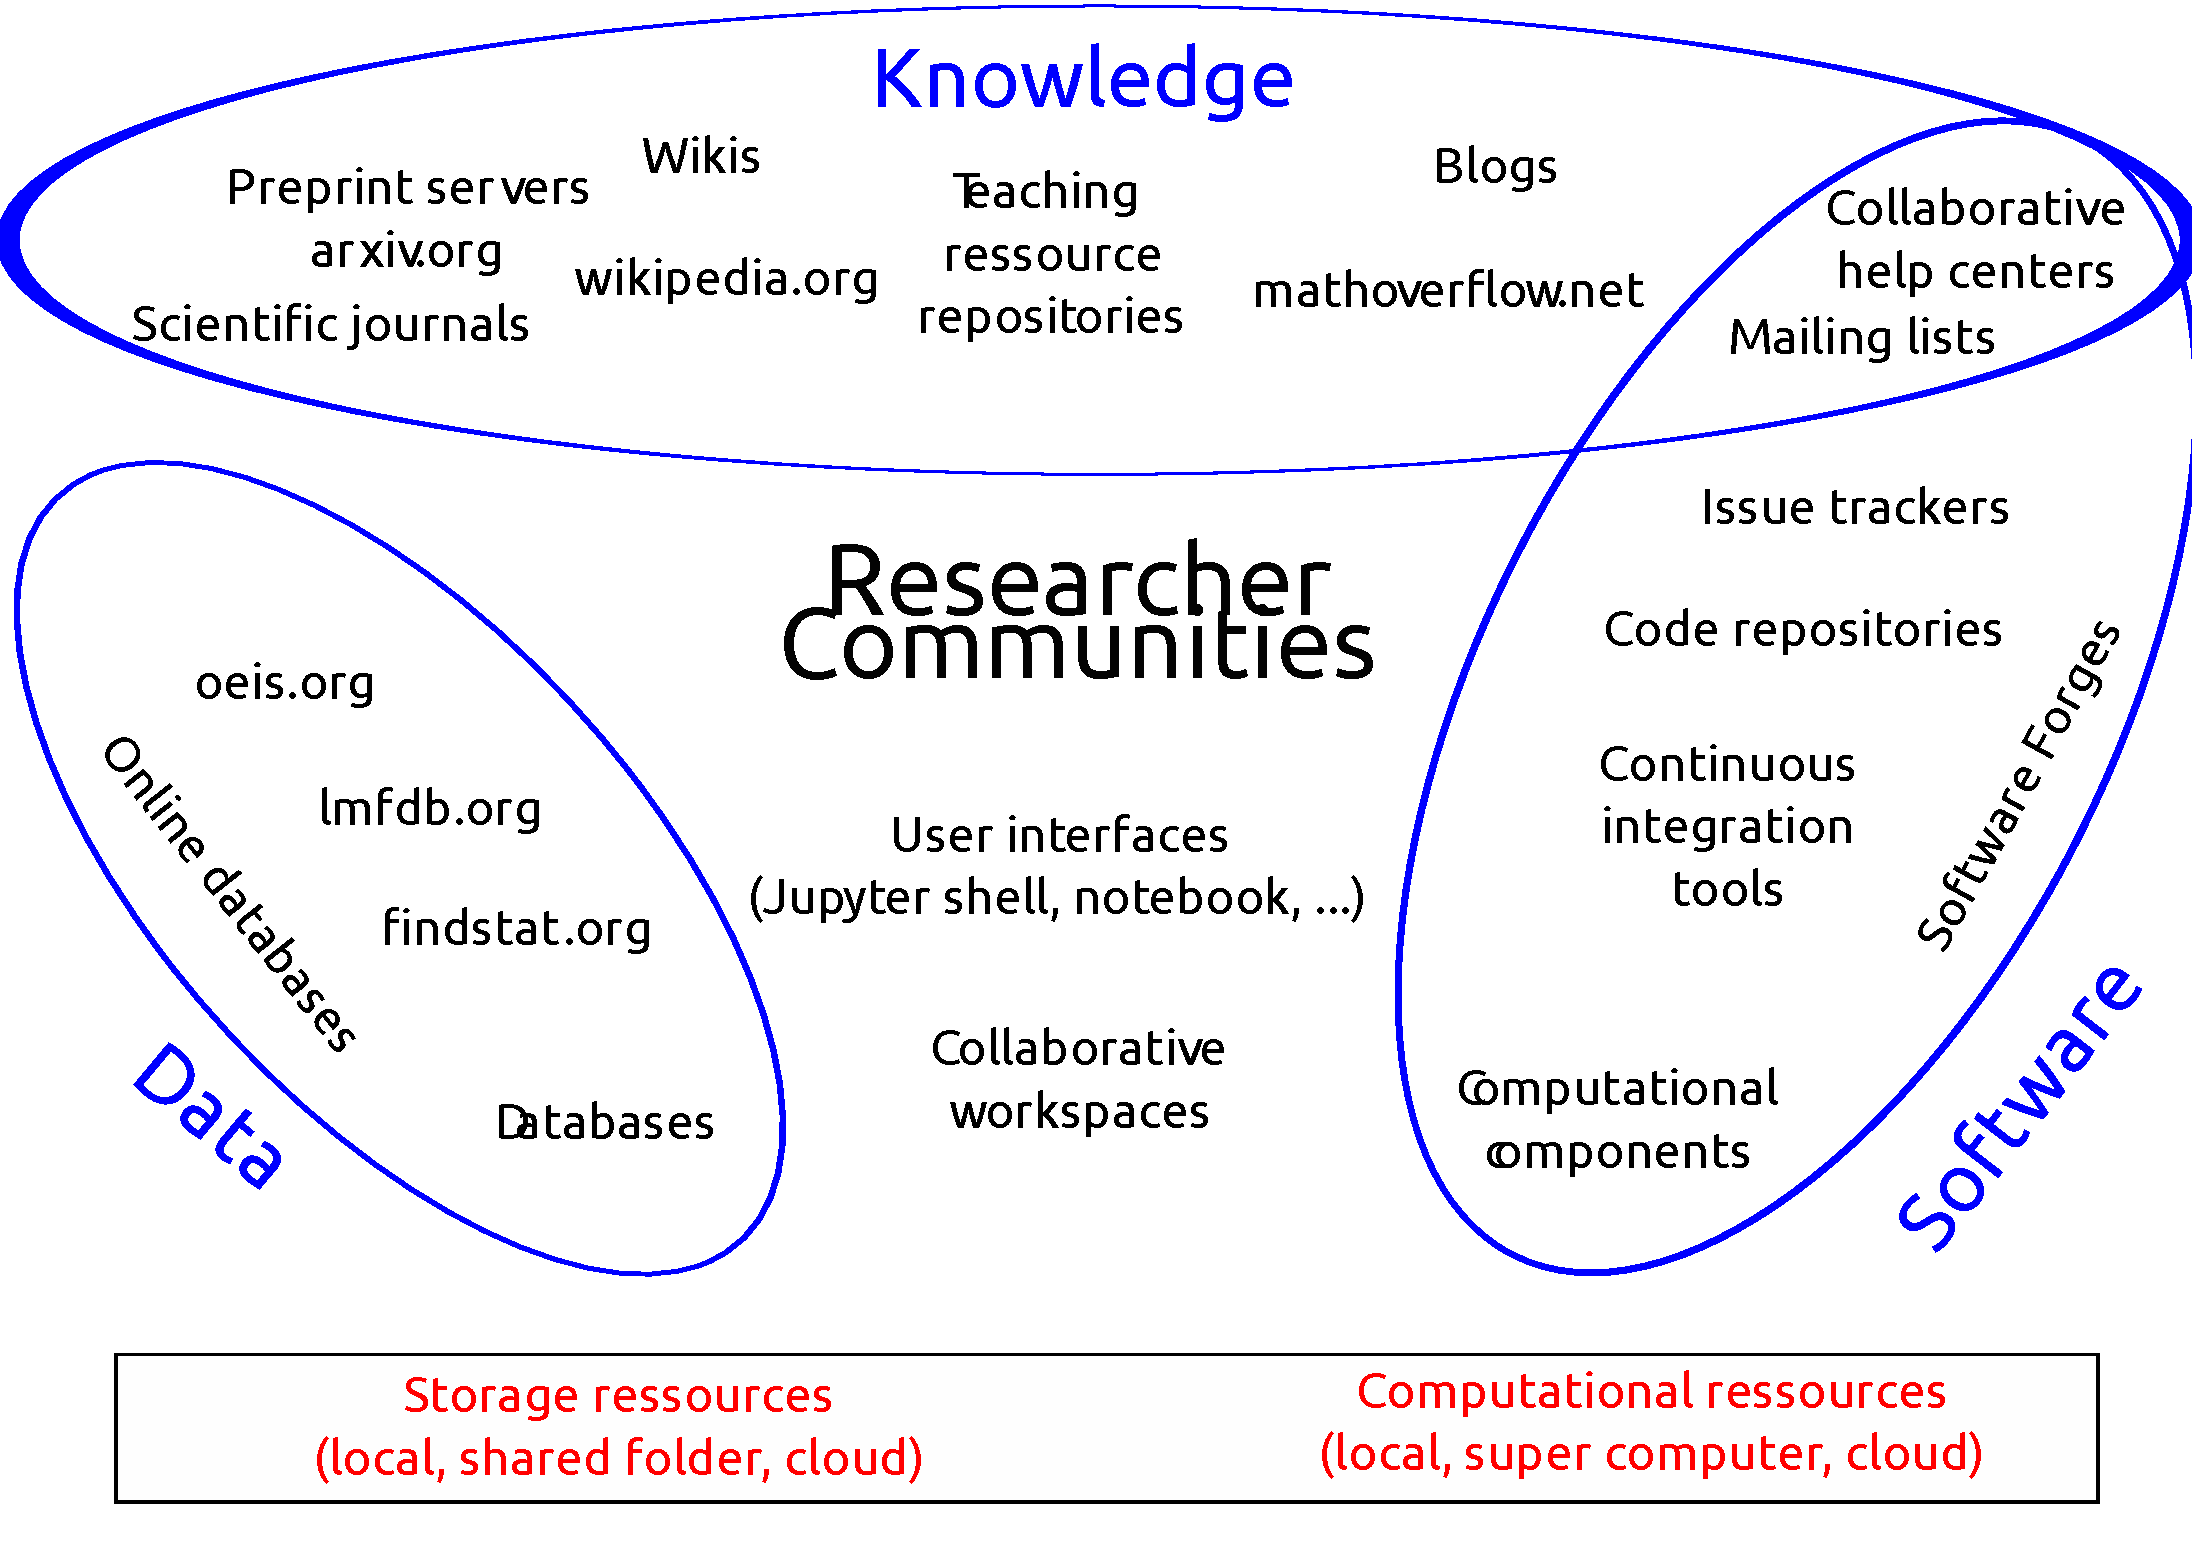
\includegraphics[width=\textwidth]{Pictures/TheBigPicture.pdf}}
  \caption{Virtual Research Environments for research in pure
    mathematics and applications.}
  \label{fig:thebigpicture}
\end{figure}

% \TODO{NT: the purpose of Figure~\ref{fig:thebigpicture} is to give a quick
%   sense of what Virtual Research Environments can be in our context,
%   and a ``big picture'' for the project. A graphic artist friend of
%   mine is going to help me improve it. I have collected here some material for her.\\\\
%   \textbf{\Large What we would like the ``big picture'' in
%     Figure~\ref{fig:thebigpicture} to highlight:}
%   \begin{description}
%   \item[This is a human centered project:] At the core: researchers and communities
%     thereof.
%   \item[The three types of information:]
%     Software, Knowledge, Data (currently in blue)\\
%     How they interact:
%     \begin{itemize}
%     \item Knowledge help structure data and software (e.g. through ontologies)
%     \item Software produce data
%     \item Data is used by researchers to build knowledge
%     \end{itemize}
%   \item[Physical resources:]
%     (currently in red)
%   \item[Virtual Research Environments]\ 
%     \begin{itemize}
%     \item Researchers in Math have a long tradition of collaborating
%       on Software, Knowledge, and, up to some point, Data
%     \item For this they use a variety of collaborative tools which
%       form a loosely knit Virtual Research Environment.
%     \item \textbf{Aim 2}: make it easy for subcommunities of
%       researchers to set up custom collaborative work spaces / Virtual
%       Research Environments tailored to their needs, by combining:
%       \begin{itemize}
%       \item Computational resources
%       \item Storage resources
%       \item Computational software components
%       \item Databases
%       \item User interfaces
%       \item Wikis-Knowledge bases (true for findstat, LMFDB): quicker
%         cycle for consolidation of information spread over
%         papers/brains
%       \end{itemize}
%       Such VRE shall help them:
%       \begin{itemize}
%       \item collaboratively develop software (e.g. specialized
%         libraries), data and knowledge (e.g. articles) for their
%         research projects.
%       \item contribute back this information to the larger community
%         whenever relevant.
%       \end{itemize}
%     \end{itemize}
%   \item[Processes:]\ \\
%     It would be interesting to depict the following processes. They
%     are indeed about collaboration and sharing (and quality control),
%     that is what \textbf{Aim 1} is to promote.
%     \begin{description}
%     \item[Software development]\ 
%       \begin{itemize}
%       \item \emph{bug reports} and \emph{enhancement requests} emerge
%         from the community, typically through collaborative help
%         centers, and are posted on issue trackers.
%       \item \emph{Design discussions} occur on mailing lists and issue
%         trackers.
%       \item Researchers \emph{submit code} to the code repositories.
%       \item \emph{Quality control}: the code is reviewed and
%         tested by continuous integration tools.
%       \item Finally the code \emph{integrated} within computational
%         components, and used by the community.
%       \end{itemize}
%       Researchers (as well as other users: teachers, engineers, ...)
%       interact at each step of the process.
%     \item[Scientific publication]\ 
%       \begin{itemize}
%       \item researchers submit articles to journals and post them on
%         preprint servers;
%       \item the articles get reviewed by other researchers;
%       \item finally they are distributed back to the community
%       \end{itemize}
%     \end{description}
%   \end{description}
%   %
%   Improvements to implement:
%   \begin{itemize}
%   \item the findstat link does not work for me, kerning looks
%     extremely weird -- POD
%   \item LMFDB, OEIS, and findstat have a strong knowledge component as
%     well, with knowls and wikis, references, ...
%   \item arxiv is not far from a database of knowledge
%   \end{itemize}
%   %
%   \textbf{\Large A collection of links that might give some idea of
%     the look and feel of our universe:}
%   \begin{description}
%   \item[Examples of (computational) components:]\ 
%     \begin{itemize}
%     \item IPython: \url{http://ipython.org/}
%     \item GAP: \url{http://www.gap-system.org/}
%     \item Singular: \url{http://www.singular.uni-kl.de/}
%     \item Sage: \url{http://sagemath.org/}
%     \item \PariGP: \url{http://pari.math.u-bordeaux.fr/}
%     \item Linbox: \url{http://www.linalg.org/}
%     \end{itemize}
%   \item[Examples of online collaborative tools]\ 
%     \begin{itemize}
%     \item Issue tracker: \url{http://trac.sagemath.org/timeline/}
%     \item Code repository: \url{https://github.com/}
%     \item Collaborative help center: \url{http://ask.sagemath.org/}
%     \item Collaborative math site: \url{http://mathoverflow.net/}
%     \end{itemize}
%   \item[Examples of online databases]\ 
%     \begin{itemize}
%     \item Online databases: \url{http://oeis.org/?language=french}
%     \item LMFDB: \url{http://www.lmfdb.org/EllipticCurve/Q/14.a3}
%     \item Findstat: \url{http://www.findstat.org/}
%     \end{itemize}
%   \item[Example of graphical material]\ 
%     \begin{itemize}
%     \item \url{http://boxen.math.washington.edu/home/nthiery/main2014.pdf}
%     \end{itemize}
%   \end{description}
% }


\COMMENT{Role of this section: reflecting our knowledge of the context
  + and explaining that the success of those early VRE’s, even if
  incomplete, showcases their importance and the appetite of the
  community for these kind of tools. It's exciting. We want to
  highlight the appetite rather than the need which is hard to define
  at this point}

\begin{center}
  \begin{boxedminipage}{.95\textwidth}\em
    \COMMENT{In short: maths needs VRE's}

    Our priority is the delivery of complete Virtual Research
    Environments (VRE). A VRE supports the entire life-cycle of
    computational work in mathematical research, from initial
    exploration to publication, teaching, and outreach. We envisage
    VREs as the main medium for development and deployment of
    mathematical research.
  \end{boxedminipage}
\end{center}

Virtual Research Environments are flexible, powerful, unified
environments for communication, distribution and implementation of
mathematical research.

Initial work shows the potential for this idea, for example, the
Virtual Research and Teaching Environment \SMC hosting more than 10k
users and 100k projects after just one year).  \TODO{Short description
  of SMC + link to the section + screenshot}

There is widespread community interest in well-executed
\emph{integrated solutions} which can enable large-scale collaboration
on Mathematical \emph{software}, \emph{knowledge}, and
\emph{data}. This interest is also evidenced by the considerable
activity (since the inception of the internet) in a range of online
mathematical databases such as the Online Encyclopedia of Integers
Sequences, the Atlas of Finite Group Representations, and \LMFDB.
%
Other systems such as \href{http://polymathprojects.org/}{polymath}
and \href{mathoverflow.net}{MathOverflow} show the interest among
mathematicians in exploring new forms of collaboration, in particular
when the tools are well-designed and the balance of effort and reward
is correct.

\TODO{Mention as well everyday's collaborative tools like arxiv,
  Wikipedia, github, each showing some aspects of VRE.}

\TODO{Simulagora}

\TODO{Highlight some other deployed VRE's that would benefit to the
  sorts of improvements you suggest.  You could include Wakari.io and
  also the tmpnb thing in Nature magazine:
  http://www.nature.com/news/ipython-interactive-demo-7.21492}

\TODO{Reference paragraph 1 of ambition for the typical sharing of
  papers/code/… through version control, but that's a minority}


\paragraph{The diversity of needs in the mathematical community}

Certain scientific areas, for example in genomics, have large
communities of researchers whose computational workflows are very
standardized, which justifies the development of specialized Virtual
Research Environments, typically taking the form of clickable web
services. The situation is very different in mathematics.

Indeed, mathematical research projects and teams that make use of
computation databases or collaborative tools are extremely diverse, in
size, skills, sophistication, needs, requirements, and available
resources. Here are some typical scenarios to illustrate this:
\begin{itemize}
\item At one extreme a project might consist of a single researcher, with limited
  general computing expertise, using a computational tool to compute some data
  that confirms or refutes a hypothesis, writing up the results as a paper
  linking to the data and publishing it. Such a user needs a simple system
  that supports the computational tool of their choice, logging and replay of
  the computation, automatic incorporation of key data in a mathematical
  document, data archival and subsequent citation. They will use very little
  computational resource, and probably have no means of paying for what they
  do use, and will have limited ability to install software.

\item A typical research project in Algebraic Combinatorics involves
  two or three researchers of varying computing skills. It will
  require tools from very different areas of mathematics: typically
  linear algebra, commutative and non-commutative algebra, symbolic
  manipulations, group theory, graph theory, language theory, and
  rewriting techniques. They thus need to use simultaneously many
  computational components, and implement a private library of code
  that combines them in novel ways. They often will have access to
  some local or remote computational resource (cloud or HPC server),
  and parallelization and distribution of the computations is
  essential to cope with combinatorial explosion. Last but not the
  least, they need to visualize the results, typically large graphs
  with complicated information on the node or edges, and may have
  access to wall-sized screens for this. They will advertise their
  results through lectures involving live demos. Early on, they will
  want to share their code and data with colleagues typically with
  little computing expertise, and eventually contribute it back to the
  community.

\item A larger collaborative project might involve five or six researchers at two
  or three sites, developing a significant extension to a system such as \Sage
  and using it to explore or catalogue examples of the mathematics of
  interest, and publishing multiple versions of their software and data, and a
  number of mathematical papers based upon that data. They need a much more
  sophisticated environment, including communication and collaboration tools,
  software development tools and so on.

\item Still another type of project would be a very large and open-ended
  collaborative framework such as polymath, but with the capability to attach
  computations, machine-checked proofs and other computational elements to the
  discussion and the collaboratively assembled proof. These are just a few of
  the many forms of computational or collaborative mathematical project that
  we aim to support.
\end{itemize}
\TODO{Add more scenarios? E.g. usage by engineers, typically to
  include Wolfram's comment about having a large array of tools under
  hand; highlight the variety of needs in term of
  data/knowledge/software}

\TODO{Another specific challenge in mathematics comes from the vast
  yet tightly connected array of concepts involved. The natural
  ontologies of mathematics are richer, more complex, and more
  interconnected than for, say, fluid dynamics.}

\subsubsection{Key concept: a Virtual Research Environment Toolkit}

As we have seen, due to the high diversity of needs in Mathematics,
there is no hope for providing a one-size-fits-all Virtual Research
Environment, not even for reasonably sized subcommunities. Instead,

\begin{framed}
  Toward an Open Digital Research Environments Toolkit for the
  Advancement of Mathematics.

  \TheProject proposes to deliver a flexible \textbf{toolkit} that
  will make it easy for individuals and teams of researchers of any
  size to set up custom collaborative Virtual Research Environments
  tailored to their specific needs, resources and workflows, which
  will provide modern, flexible and reliable support for the entire
  life-cycle of computational and collaborative work in mathematical
  research, from initial exploration to proof, publication, archival,
  teaching and outreach. They will support mathematical computations
  and databases of all scales from tiny to huge.
\end{framed}

The kit will take the form of a collection of compatible components,
ready to be connected using extensible documented interfaces both to
other bespoke components and to standard infrastructural tools and
services. Most of the capabilities of these components will come from
existing software -- computational tools such as \Sage, \GAP,
\Singular and \Pari; databases such as \LMFDB; user interface tools
such as \Jupyter notebooks; existing compute servers, clusters and
clouds; typesetting tools such as \LaTeX\ and so on.

\paragraph{First benefit: meeting actual needs in Mathematics}

The kit will be designed to create VREs that support the ways in which
mathematicians actually work together through the lifecycle of a
project, informed by recent research into the sociology of
mathematical collaboration.

Engineering the social aspects of such systems to maximize their
success is an imprecise science. A great deal is learnt from the
deployment of any given system and the reaction of the wider
community. Historically setting up these infrastructures has required
massive efforts: \SMC required 70k lines of
bespoke code; similarly each of
the databases and collaboration sites is essentially a bespoke
program. Unfortunately much of the effort is necessarily \emph{not} on
the innovation in the environment, but on the underlying
infrastructure. To ensure focus can be placed on the environment
itself we require a more flexible and reusable system. Its
characteristics must include portability, compatibility, performance,
usability, and reproducibility. It should bootstrap our understanding
of the social dynamics of user and developer communities.

\subsubsection{Approach}

In the previous section, we have analyzed the diverse needs of
researchers in pure mathematics and applications, and argued that the
concept of a VRE toolkit, as proposed by \TheProject, will match those
needs, and have a considerable impact on how mathematical research is
conducted.

We now explain our approach to implement this concept, and argue why
now is a critical point providing an opportunity to do so.
\begin{framed}
  The fundamental factor is that the last decade has witnessed the
  emergence of the necessary building blocks, all in open source:
  \begin{itemize}
  \item Key technologies: virtual machines and containers for easy
    deployment, cloud infrastructure like open stack, web technologies
    like Mathjax or WebGL for powerful in-browser clients, scalable
    decentralized database software, ...
  \item Computational mathematics components
  \item User interfaces and interactive computing environments
  \end{itemize}
\end{framed}

This emergence was enabled by the maturation of open source
development models and collaborative tools (e.g. \texttt{github}) that
now allows for bringing together very large and diverse communities of
developers, and fostering large ecosystems of interoperable
components. We elaborate later in this section how this has
specifically affected the development of mathematical software in the
last decade, showcasing the sustainability of the ``by users for
users`` development models even for general purpose mathematical
computational components.

\SMC proves the feasibility (but 70k of code).


\begin{frame}
  Our approach is to join forces with \Jupyter and focus on developing
  and improving building blocks of e-infrastructure that can be
  assembled and re-used flexibly to address a wide range of
  requirements in mathematics and the applications of mathematics in
  science and engineering, rather than creating one particular
  monolithic environment.

  and built out of a sustainable ecosystem
  of % both domain-specific and general purpose
  community-developed open software, databases, and services.
\end{frame}

Throughout this project we will reuse and extend open source code, and
\TheProject will benefit from future open source contributions during
and beyond the lifetime of the project. By unifying tools with
overlapping functionality, such as \Jupyter and \Sage, we focus the
effort of the computational community onto \TheProject, producing
additional economies of scale. Finally, thanks to the ``by users for
users`` model, the development will be steered by the actual needs of
the community.

\TODO{Explain the high return on investment.}

\subsubsection{Activities}

The activities of the project are planned and structured to develop
and promote \TheProject, including new research into
architectures, database techniques, parallel algorithms and the
sociology of collaborative free software development, as well as
engineering work on existing software and networking and
community-building activities.

The project inherently spans the disciplines of mathematics and
computer science, as well as bringing in results and techniques from
social sciences. Exemplar applications may also arise from areas to
which symbolic and algebraic computing is applied, such as physics,
chemistry, systems biology and engineering.


The project is divided into seven work packages. Work Package
\ref{management} covers project management and coordination as
usual. Work Package \ref{dissem} is our main Networking activity
including community-building workshops, demonstrator applications and
direct dissemination of project results.
This covers the following topics from section E of the Work Programme:
\begin{itemize}
\item  dissemination and/or exploitation of project results and knowledge, contribution to socioeconomic
impacts, promotion of innovation ;
\item reinforcing partnership with industry: outreach and dissemination activities, transfer of
knowledge, activities to foster the use of e-infrastructures by industrial researchers,
involvement of industrial associations in consortia or in advisory bodies;
\item strengthening of virtual research communities;
\item spreading of good practices, consultancy and training courses to new users;
\item exchange of personnel and training of staff;
\end{itemize}

\TODO{reference specific tasks for each bullet-point}

The remaining work packages are Joint Research Activities, dividing up
the research needed to design and implement the \TheProject and
investigate the best models for its future development. \TODO{Explain
  the rationale for the division and how they all come together at the end}

This covers the following topics from section E of the Work Programme:

\begin{itemize}
\item higher performance methodologies and protocols, higher performance instrumentation,
including the testing of components, subsystems, materials, techniques and dedicated
software;
\item integration of installations and infrastructures into virtual facilities;
\item innovative solutions for data collection, management, curation
  and annotation;
\end{itemize}

\TODO{tasks or WPs}

Additional topics addressed include effective software development and
maintenance methodologies for systems of free software systems and the
design of VREs to best support real mathematical practice.

Since the infrastructure that we are developing is free software,
there is no need for formal Service activities. All partners have
access to all the software anyway, and development and demonstration
can take place on computers already available to the partners. 

\subparagraph{Networking activities}
\TOWRITE{}{how the workshops etc are carefully planned to bring everyone together, existing
  great culture, etc.}

\subparagraph{Joint Research Activities}
\TOWRITE{}{here is probably where we say why these are the exact topics that
  need work if DreamKit is to happen and repeat how much more
  wonderful it will be than just using existing software. Some kind of
description of the software architecture probably belongs here}

Combining this with the.

improving those building blocks in order to make it easy to combine
them. Some of them need to be updated to run to best effect in modern
environments, most will need adaptation to support the \TheProject
interfaces. Some new components may be needed. Groundwork must also be
laid for effective consistent maintenance and future development of
these components.
  
\TOWRITE{NT}{Where to put the list of demonstrators}
\subsubsection{Demonstrators}
\paragraph{Micromagnetic VRE}
\label{sec:introduction-micromagnetic-vre-demonstrator}

\begin{figure}
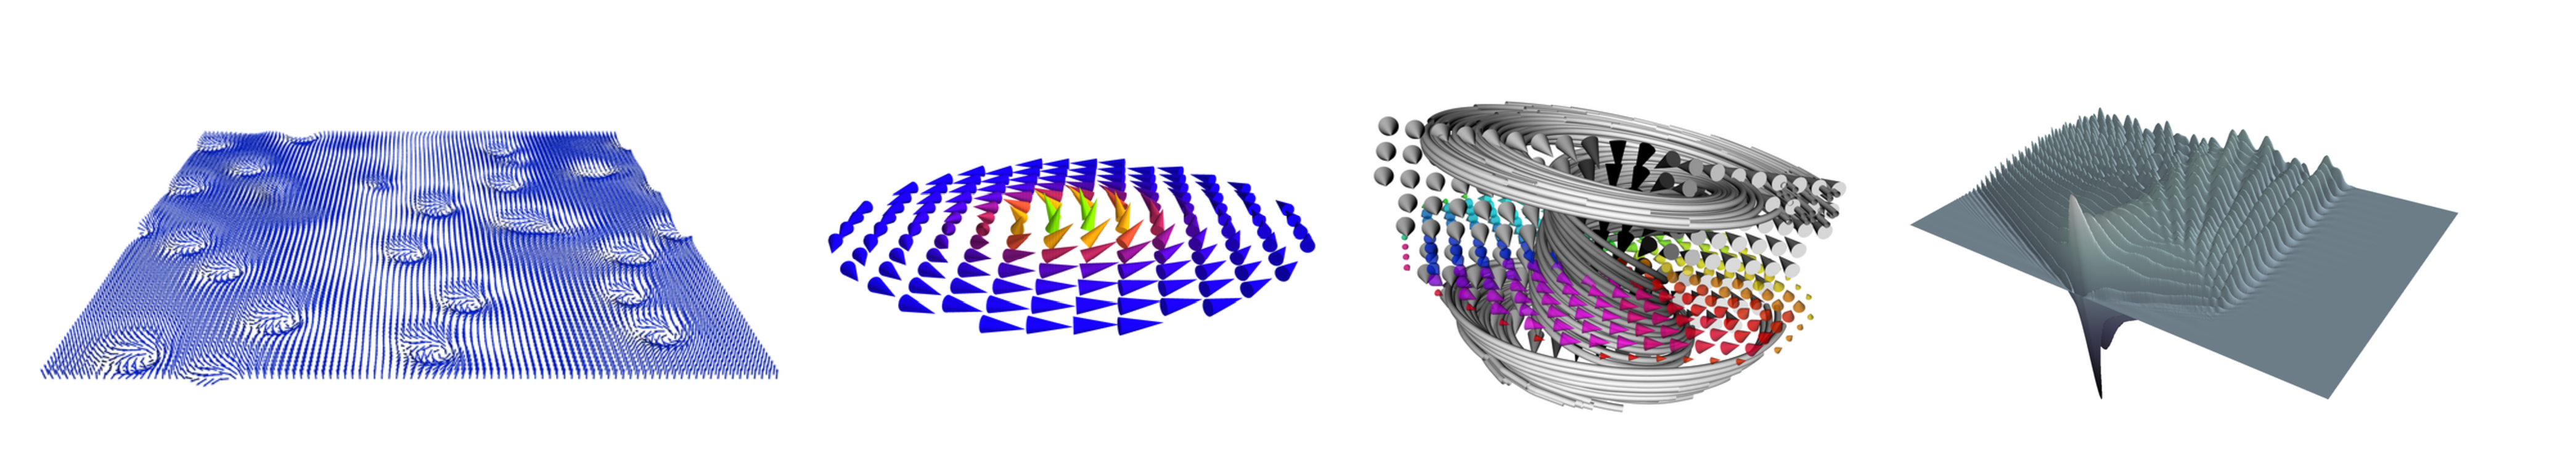
\includegraphics[width=1.0\textwidth]{Pictures/micromagnetic-and-3d-vis-4x1.pdf}
\caption{\label{fig:3d-plots} A selection of typical visualisation patterns often required in science and engineering. From left to right: a 3d vector field on a 2d domain, a 3d vector field coloured with another scalar field on a 2d domain, a 3d vectorfield on a 3d domain with streamlines, and scalar field plotted on a 2d domain.}
\end{figure}

Micromagnetics is a continuum theory description of the behaviour of
the magnetisation vector field at length scales of the order of
micrometers and below. It is widely used in the research and
development of magnetic data storage media and devices, for magnetic
sensing, permanent magnets and healthcare applications such as cancer
treatment and diagnostics. The mathematical model is a time dependent
nonlinear partial differential equation with multiple length and time
scales in the problem, and solution strategies are based on finite
difference and finite element space discretisations and sophisticated
numerical solution of the equations. As in many other research fields,
the groups carrying out the simulations are often not the code
developers, nor have they extensive computational background. More
commonly, these are material scientists, engineers and physicists that
use the simulation to interpret their experiments and support their
device design planning. Industrial users include Seagate, Hitachi,
TDK, Samsung, Bosch and Toyota.

Figure~\ref{fig:3d-plots} shows magnetisation vector fields obtained
in typical micromagnetic studies. They relate, from left to
right, to a set of interacting magnetic skyrmions in a thin flim, a
vortex in a thin Nickel film, a vortex in a half-sphere geometry, and
the propagation of magnetic excitations (only one component plotted)
in a 1d-system.

In this project, we will use the \TheProject components to put
together a in micromagnetic VRE to (i) demonstrate the power of the
approach in a concrete applied research setting, (ii) exploit that
experience to evaluate the real value of the structure of this VRE and
\TheProject to a large and diverse set of end-users.

In more detail, we will embed the most popular micromagnetic
simulation software: the Object Oriented MicroMagnetic Framework
\cite{OOMMF-url} within a micromagnetic VRE, complement this with
value-adding features, develop a substantial number of executable
documents inside this VRE that act as tutorials and documentation,
disseminate the software and documents as open source and through
workshops for the micromagnetic community.  

We have chosen the OOMMF simulation package as the target tool because
it is a somewhat typical representative of computational software:
computation is driven through a text-based configuration file, data
files are produced, and later processed, then figures are created from
the processed data; leaving the scientist with the burden to link all
these elements together. The benefits of moving to the integrated
notebook workflow (see Section~\ref{sec:jupyter}) are
substantial. Furthermore, OOMMF is widely used (over 1800 recorded
publications \cite{OOMMF-citations-url}) and thus provides benefit to
an active and substantial community, who in return will provide plenty
of feedback.

We evaluate the value of this demonstrator
(\taskref{social-aspects}{oommf-nb-evaluation}), immediately feeding
results back into the \TheProject work. This will also
be a case study for the sustainability of the approach and tool beyond
the life time of this H2020 project.




\TODO{explain what kind of improvements:
  \begin{itemize}
  \item faire ce qu'il faut pour pouvoir composer les composants de
    calcul et les rendre portables et performants sur une large gamme
    d'infrastructures.
  \item Improve \Jupyter
  \item 
  \end{itemize}}

\TODO{reference for sustainability}

\TODO{Recycle stuff below and advertise the last section on maximising
  sustainability and impact}

\TODO{Key factor: development models and communities that want to
  collaborate}


\paragraph{Development models for mathematical software: a historical
  perspective}

\COMMENT{Goal: discussion about development models for mathematical software}

Supporting the experimental method requires spending major efforts
on software development. As the sophistication of the required
computations increased, supported by the boom of the available
computational power, it became vital to share those efforts at the
scale of large research communities. European mathematicians have been
pioneers and have grown a steady tradition of collaborative open
source software development, with specialized systems like \GAP,
\Singular, or \PariGP playing a major role for decades.

\TODO{fuse those two paragraphs}

Collaborative software innovation by mathematical researchers was key
to the development (often in Europe) of many highly successful,
open-source, community-developed specialized systems, starting with
\PariGP in Number Theory in 1979, and including \GAP in Group Theory
or \Singular in Algebraic Geometry. This was at a time when much other
scientific computing research relied on bespoke Fortran programs used
for one calculation and then discarded.
%  \TODO{Is this quite true?
%  \url{http://en.wikipedia.org/wiki/Basic_Linear_Algebra_Subprograms}
%  says BLAS dates back from 1979 as well.}

\COMMENT{The emergence of massive collaborative development models and
  tools is revolutionizing the landscape; innovation is now led by
  communities, not corporate software}

\TODO{There is redundancy below}

In that period inter-project communication was limited by the lack of
interconnection between computers, leading to systems remained limited
to specific research topics and non-interoperable. It was left to the
corporate world to gather sufficient manpower to develop general
purpose systems, that could support a broad range of engineering,
scientific and statistical mathematics, through a coherent user
interface. These companies (e.g. Wolfram, Mathworks, MapleSoft) were
mainly US-based and created a profitable industry.

% The next scale was reached in the last decade with the advent of the
% general purpose mathematical system \Sage which proved the viability
% and sustainability of the ``developed by users for users'' development
% model at the international level.

The modern environment, however, is quite different. A more connected
digital world has led to the emergence of \Sage. \Sage is a truly
general purpose computational mathematical system. It is committed to,
and draws huge benefits from, the power of open source software a
virtual software development environment. It showcases the modern
reality that open source software is not just a viable alternative for
commercially produced alternatives, but it actually allows for more
rapid innovation through providing an open platform through which the
community can deploy and share advances more rapidly. \Sage showcases
this modern user-driven community approach to development by
delivering high quality software to researchers, teachers, and
practitioners in mathematics. It is founded on a widespread
international community of contributors and developers and builds
successfully on a large stack of existing open source software,
ranging from the specialized computational systems mentioned above, to
\Python, a general purpose programming language that is used by
millions of programmers worldwide. This flexible, open source
architecture then allows it to rapidly assimilate new components such
as \Jupyter (formally IPython notebook) as they are developed.

In the 1980s and 1990s the economies of scale favoured the commercial
development model for mathematical software: corporate entities could
co-locate a large body of expertise and orient it towards one
goal. This was difficult for the much larger, but naturally more
dissipated, communities of mathematical researchers. However, modern
interconnection of researchers (through the infrastructure of the
internet and collaborative development environments such as github)
means that the balance of these economies of scale has been
reversed. Commercial packages can no longer develop fast enough to
assimilate the innovation of the wider mathematical community, where
there is greater expertise and manpower.

\TODO{The material here is somewhat redundant with the language in
  Objective~\ref{objective:sustainable}; see where this belongs best
  to. The previous section being too long, it might be good to move
  things here.}

\paragraph{A unifying concept: executable notebooks}

A key technology here is \Jupyter (formerly
\IPython), a set of open-source software projects for interactive and
exploratory computing. These software projects help make scientific
computing and data science reproducible and multilanguage (\Python,
Julia, R, Haskell, etc.). The main application offered by Jupyter is
the Jupyter notebook, a web-based interactive computing platform that
allows users to create data- and code- driven narratives that combine
live code, equations, text, interactive dashboards and other rich
media into a single executable document. \Jupyter is already used very
widely in research and development, both in academia and industry and
the user base grows rapidly.

\TODO{Here could be a good spot to cite \href{https://www.authorea.com/users/23/articles/8762/_show_article}{The Paper of the Future}}

\paragraph{Maximizing sustainability and massive impact}

By focusing on a toolkit rather than a monolithic VRE, and by
concentrating the efforts on improving and unifying existing general
purpose building blocks, and in the forefront \Jupyter, \TheProject
will simultaneously maximize sustainability and broad impact. Indeed,
even if the primary target users are \emph{researchers in
  mathematics}, the set of beneficiaries extends to scientific
computing, physics, chemistry, biology, engineering, medicine, earth
sciences and geography, and include researchers as well as teachers
and practitioners in the industry. \TheProject will further foster
development models that are mutually beneficial to academia and highly
innovative SME's.

\COMMENT{Even just the improvements of the components themselves will
  have a strong impact}

\subsubsection{Answers to specific requests of the call}

\paragraph{Use of Existing Basic Services}
\TOWRITE{}{This is a possible weak point -- does anyone know anythign
  about this}

\paragraph{Gender analysis}

All partners will follow inclusive practices in recruiting staff for
this project, in inviting the community to our workshops and outreach
events and in choosing users to evaluate our demonstrator
applications. We will consult with \TODO{someone -- could be the Head
  of Equality and Diversity at St Andrews if you like, or one of UMs
  sociology friends} about any known gender differences in
collaborative working and ensure that our collaborative tools properly
support open, equitable and inclusive patterns of cooperation. 
\TODO{say that we'll report this in some deliverable}.


 \TheProject aims to create a framework to make the
systems interoperable and synergistic and to give working mathematicians full access to
the potential spanned by already-existing systems. Essentially every node in
Figure~\ref{fig:thebigpicture} represents a user community, so \TheProject is at its heart
a project that also combines researchers and communities.


\subsubsection{Old material}

\TODO{What the proposal is about}
This proposal is about providing mathematicians with the tools to
carry out and communicate their research effectively. It will ensure that ideas are
distributed and discussed as widely as possible to enable rapid
assimilation of these ideas into the pipeline of innovation. Our aim
is to develop an ecosystem that exploits the modern computing
infrastructure to streamline development and deployment of
mathematical advances. We will ensure that the societal benefit of
these advances is realized in the shortest possible timescale.

This proposal is about supporting the next generation of innovation in
the mathematical computing ecosystem. It is a Europe-wide
collaboration that assimilates a leading body mathematicians and
computational researchers with a track record of delivering innovative
open source software solutions.

In keeping with the \Sage strategy, a major focus is on reusing and
improving existing components, and reaching toward larger communities
whenever possible. 

\begin{center}
  \begin{boxedminipage}{.95\textwidth}\em
    \COMMENT{Short description of the consortium}

    To achieve this aim, \TheProject brings together lead developers
    and experts from existing mathematical computational components
    (\Linbox, \GAP, \Sage, \Singular), existing Virtual Research
    Environments (\SMC, \Simulagora), online mathematical databases
    (\LMFDB), mathematics knowledge portals (\MathHub) and general
    purpose interactive computing components (\Jupyter).

    \TODO{Most of the participants are themselves primary users of the
      infrastructure, with a long track record of community building
      and dissemination. Thus the governance will naturally be steered
      by users needs.}
  \end{boxedminipage}
\end{center}


  Chunks of language that we might want to recycle above:
  \begin{compactenum}[\em i)\rm]
  \item \TheProject will attack all those challenges upfront, while
    consolidating Europe's leading position in this field.
  \item innovate virtual research environment (VRE) development:
    instead of building an essentially monolithic system like
    Mathematica or Maple, we will build an open framework for Math
    VREs, which can be extended by plugins and experimented on as
    needed, and
  \item wrest the initiative in the space of computational mathematics
    from the corporate world into the open source research/innovation
    community, which is traditionally strong in Europe.
\end{compactenum}

\subsubsection{Linked research and innovation activities}\label{linked-projects}

\eucommentary{Describe any national or international research and
  innovation activities which will be linked with the project,
  especially where the outputs from these will feed into the project;}

\TODO{For each item below, write a paragraph describing the project
  and one describing how it connects with this proposal}

\paragraph{DFG Priority Project SPP 1489}
\url{computeralgebra.de}

The SPP1489 ``Algorithmic and Experimental Methods in Algebra, Geometry, and
Number Theory'' is a nationwide Priority Project of the German Research Council DFG  
which commenced in July  2010 and will end in June 2016. The focus of the programme 
is on the interactions between computer algebra and algebraic geometry, number theory, 
and group theory. It combines expertise at all levels of research in computer algebra, 
be it the design of algorithms, the implementation of algorithms, the application
of algorithms, or the creation of mathematical databases. The goal of SPP1489 is to 
considerably further the algorithmic and experimental methods in the afore mentioned
disciplines, to combine the different methods across boundaries between the disciplines, 
and to apply them to central questions in theory and praxis. A fundamental concern of the
programme is the further development of open source
computer algebra systems with origins in Germany, which in
the framework of different projects will be cross-linked on
different levels. Of particular interest are interactions with application areas inside
and outside of mathematics such as system- and control theory, coding
theory, cryptography, CAD, algebraic combinatorics, and algebraic
statistics as well as hybrid methods which combine numerical and
symbolic approaches. 

The work in the SPP1489 has established effective communication channels between 
the core developers of different computer algebra systems. It is a showcase project
for several objectives of this proposal (such as community building and
fostering a sustainable ecosystem of interoperable open source components). 
The experience made in parallelizing mathematical software will be crucial for
Work package WP5.


\paragraph{IPython/Jupyter grant from the Alfred P. Sloan foundation}
\url{http://ipython.org/sloan-grant.html}

The IPython project received a \$1.15M grant from the Alfred P. Sloan%$
foundation that is supporting IPython development for two years
(1/1/2013-12/31/2014), in particular at the University of California,
Berkeley and California Polytechnic State University, San Luis Obispo.
This grant enabled the project to focus on developing the IPython
Notebook as a general tool for scientific and technical computing that
is open, collaborative and reproducible. This goes a long way toward
Aim \TODO{... and ...} of \TheProject, especially given the current
rapid evolution of IPython toward its language agnostic avatar
Jupyter.

\TheProject will build on the outcome of the Sloan grant, and further
develop the critical IPython/Jupyter component in close collaboration
with the IPython/Jupyter team. In particular, we plan to hire some of
the European developers that are currently funded by the Sloan grant
to work in California and wish to later return to Europe.

\paragraph{NSF SI2-SSE OCI-1147247}

%\SageCombinat is a subproject of \Sage whose mission is "to improve
%\Sage as an extensible toolbox for computer exploration in (algebraic)
%combinatorics, and foster code sharing between researchers in this
%area".

The OCI-1147247 Collaborative Research grant ``Sage-Combinat:
Developing and Sharing Open Source Software for Algebraic
Combinatorics'' is a project funded by the National Science Foundation
from June 2012 to May 2015. The grant supports the development of
\SageCombinat, on the USA side, and in areas relevant to the ongoing
research of the participants (symmetric functions, Macdonald
polynomials for arbitrary Cartan types, crystals, rigged
configurations and combinatorial R-matrices, affine Weyl groups and
Hecke algebras, cluster algebras, posets, ...), together with relevant
underlying infrastructure. The grant funds a yearly Sage Days
workshop, and cofunded two others at ICERM and Orsay respectively. The
grant also funds a dedicated software development and computation
server for \SageCombinat, hosted in the \Sage computation farm in
Seattle. Emphasis is placed on the development of thematic tutorials
that make the code accessible to new users. The grant also funds
graduate student RA support, curriculum development, and other
mentoring.

Two of the proposers, Stein and Thiéry, are respectively PI and
foreign senior participant to this NSF grant. It funded, through them,
some of the development of \SMC as well as of the category framework
in \Sage; both are key assets for this proposal. The workshop and
outreach actions pursued by this NSF grant have proven to be potent
tools for connecting researchers and recruiting users and
developers. One of the role of this proposal is to support similar
community building in Europe.

\paragraph{HPAC grant from the A.N.R.}

The French national research agency ANR has funded a 4 years project
on High Performance Algebraic Computing (HPAC) focused on the
development of parallel exact linear algebra. The consortium gathers
research groups from LIP6 (Paris 6), LIRMM (Montpellier), LIP (Lyon)
and LIG and LJK (Grenoble). The main goals of the project is to first
develop high performance exact linear algebra kernels with dedicated
parallel runtime, propose a domain specific language for the
parallelization of exact linear algebra libraries and their
composition, invent new algorithmic solutions for large scale
parallelizations. The output of the project is then twofolds: new
computational challenges arising in algebraic cryptanalysis will be
addressed, and the open-source libraries maintained by each group will
not only integrate these advances, but will expose them in a close
integration to high level computer algebra softwares. In this process,
\Sage will start benefitting from the new shared-memory parallel code
of \Linbox for the linear algebra over a finite field.  The scope of
this project is mostly focused on shared memory parallelism (except
for some challenge computations). Addressing distributed and
heterogeneous infrastructures is the next step after this project,
that is be addressed in work-package 5 of the this proposal.


\paragraph{RADIANT Grant from EU FP7-HEALTH (ref 305636)}
\url{http://radiant-project.eu/}

This EU funded proposal focuses on making available computational and
mathematical models to the computational biology communities as
rapidly as they are developed with a particular focus on high
throughput sequencing techniques. The rapid development of sensorics
technology in the biological sciences results in mathematical
challenges in the data analysis. To address these challenges in a
timely manner collaborative frameworks for mathematical and
computational modelling are required. \TheProject provides the
framework for pipeline delivery of methodologies to end users through
approachable IPython/Jupyter notebooks.

% for an example see: http://nbviewer.ipython.org/github/SheffieldML/notebook/blob/master/compbio/index.ipynb

\paragraph{Cubicweb} \url{http://www.cubicweb.org}

Logilab has been developing CubicWeb since 2001 as FLOSS (Free Libre Open
Source Software). CubicWeb is a semantic web framework, that allows to
build web applications and web services from an ontology. CubicWeb
could be used in \TheProject to build mathematical databases dynamically
that will store data, knowledge and software.

\paragraph{Simulagora} \url{http://www.simulagora.com}

Logilab is maintaining Simulagora, a software as a service (SaaS) that builds
on free software (FLOSS) to provide its users with a Virtual Research Environment
(VRE) that greatly guarantees traceability and reproducibility as well as
facilitates group collaboration. Logilab will bring its experience of Simulagora
to \TheProject and feed back to Simulagora many of the deliverables available
under a free license.

\paragraph{Sage Math Cloud} \url{https://cloud.sagemath.com/}

\SMC provides a collaborative online environment for students,
teachers and researchers to interact with \Sage and with each
other. It has \Sage and \IPython worksheets, powerful \LATEX editing
features and a full \Linux computer, all accessible from a standard
web browser. Its main design feature is to enable and promote
collaboration between groups of users. It is for example a natural
place to host a course, allowing teachers to collaborate with their
students using modern tools like \Sage and \LATEX, with facilities for
real-time communication through chat, video, and shared editing of
documents, programs and worksheets; course material can be provided as
worksheets, assignments can be distributed, collected, and returned as
well. Launched in 2013, \SMC presently hosts over 100,000 projects and
10,000 weekly active users. This fast adoption by a wide variety of
users demonstrates the relevance and the long term impact this kind of
collaborative environments can have.

Technically speaking, \SMC is a specific open-source cloud-based
Virtual Research and Teaching Environment for mathematics developed
since 2013 under the lead of William Stein, with funding from the NSF,
and Google's Education Grant program.
It's currently deployed partly at the University of Washington at
Seattle, and there is a business plan for commercial support for
courses.


%  It's currently deployed at the
% University of Washington at Seattle, with a business plan in the work
% for commercial support for massive on line courses, subsidizing a free
% service for all other academic usage and some further \Sage
% development.

In comparison \TheProject focuses on open source building blocks and
architecture to easily set up and deploy custom Virtual Research
Environments. On the one hand, \SMC will serve as prototype for
\TheProject, paving the way and showcasing important features from the
users perspective. On the other hand, basically each and every task
undertaken in \TheProject will benefit back \SMC.

\paragraph{FLINT grant?}

\paragraph{LMFDB grant}\url{http://www2.warwick.ac.uk/fac/sci/maths/people/staff/john_cremona/lmf}

The L-functions and Modular Forms Database (LMFDB) project originated
at a meeting at The American Institute for Mathematics (AIM) in 2007.
L-functions are ubiquitous in number theory, and have applications to
mathematical physics and cryptography. The simplest example of an
L-functions is the Riemann zeta function. Two of the seven Clay
Mathematics Million Dollar Millennium Problems deal with properties of
these functions, namely the Riemann Hypothesis and the Birch and
Swinnerton-Dyer Conjecture, that were conjectured following
computational exploration.  As well as providing a central repository
of data as a resource for researchers, through its website
\url{www.lmfdb.org}, the LMFDB provides a modern handbook, including
tables, formulas, links and references, concerning particular specific
L-functions and their sources.  Between 2008 and 2012 the LMFDB was
funded through a US National Science Foundation (NSF) Focussed
Research Grant (FRG) of around \$1M.  Since 2013, the funding of the%$
LMFDB has passed to Europe through a six year £2.2M Programme Grant
(grant reference EP/K034383/1) from the UK Engineering and Physical
Sciences Research Council (EPSRC), held at the universities of Warwick
and Bristol, with Professor John Cremona (Warwick) as its Principal
Investigator.  This grant supports six three-year postdoctoral
research fellows, mathematical researchers who work on the
mathematical aspects of the project full-time, biannual workshops,
equipment and a portion of the investigators' own time.

Almost all contributors to the LMFDB project, including those directly
supported by the EPSRC grant and the larger world-wide team of 30-50
contributors of data and code, are pure mathematicians.  Most of these
have good computational skills, but are not professional programmers
or software developers.  The LMFDB has a great need to broaden the
support it can call upon from software developers, to enhance the
project in several ways, including the computation of number-theoretic
data but more specifically in supporting the database management and
website user interface, in order to make the data more accessible and
useful to others.  The codebase of the LMFDB project is entirely open
source and hosted at GitHub \url[https://github.com/LMFDB/lmfdb], written
in python with specialist modules such as flask and pymongo to manage
the website and database interface, and \Sage\ for higher-level
mathematical computations.  It also implements ``Knowls'', a very fruitful method of presenting mathematical knowledge.

The LMFDB project would therefore benefit
greatly from collaboration with \TheProject as it would connect the
project with a pool of experts.  Joint workshops between the LMFDB and
\TheProject will stimulate and develop such collaboration: the LMFDB
places great importance on its workshops, which are small gatherings
of around 30 invited participants who work throughout one week on
certain specific aspects of the project, coming together in plenary
sessions to make decisions, plan and collectively approve of proposed
developments.  As a leading example of the use of databases in
mathematical research, the LMFDB will provide \TheProject\ with a real
large-scale prototype around which to develop new ideas about the
design and implementation of such databases and their associated
software.  The feasibility of such collaboration was successfully
tried at a workshop at the ICMS in Edinburgh in January 2013 on
``Online databases: from L-functions to combinatorics'', sponsored by
the NSF, AIM and the ICMS.

\paragraph{Edith Elkind's ERC Starter Grant} 
``Algorithms for Making Complex Decisions on Structured Domains'' (ACCORD), 
awarded in 2014, and to be started in March 2015, 
will develop theoretic tools for analysing and improving situations
arising in collaborative environments. 
It can be viewed as a interdisciplinary project, bringing together methods from
computer science, game theory, and economics and political science
to quantify complex behaviour of social interactions, and engineer
positive outcomes by designing appropriate mechanisms.
In particular, it aims to develop a suite of preference aggregation procedures with complex outputs (i.e.,
partial orders satisfying user-defined structural restrictions) that admit efficient algorithms on realistic
inputs and are computationally resistant to dishonest behavior, and to identify a set of guiding 
principles that can be used to choose an appropriate procedure from this suite for a specific decision-making
scenario.

\TheProject\ VRE appears to be a natural testing ground and a potential virtual
laboratory for developing and testing ideas and tools developed, within the
framework of the grant, on in a ``real life'' situation, and the collaboration
will be mutually beneficial for both projects.

 
\paragraph{Ursula Martin's EPSRC Senior Fellowship grant}
``MathSoMac: The Social Machine of Mathematics'' (EP/K040251/2), started in 2014 and to be running 
for 4 years, brings rigorous methods from social
sciences into studying of the crowdsourcing, e.g. large-scale online
collaboration, phenomenon in mathematical sciences. 
 Most striking is this regard are recent large scale collaborations, such
as the Polymath projects led by Fields medallists Gowers and Tao, which used a blog to coordinate the
activities of mathematicians around the world, most recently in work on Bounded Gaps between primes; and
the collaboration led by Fields medallist Voevedsky, developing significant portions of mathematics
within the framework of new foundations based on homotopy type theory. Martin’s project will develop new
paradigms to understand these, and new tools to support them, within the framework provided by the
larger EPSRC collaboration, SOCIAM, 2013-2018. SOCIAM, a collaboration led by Nigel Shadbolt, Tim
Berners Lee and Wendy Hall at Southampton, in collaboration with Martin and De Roure at Oxford, and
Robertson in Edinburgh, aims to understand the phenomenon of social machines, defined as purposeful
human interactions on the web, and through developing unifying principles, models and tools, to enable
the effective co-ordination and deployment of the burgeoning ecosystem of social machines currently
available. The defying example of a social machine is Oxford’s Galaxy Zoo project through which
thousands of amateurs around the world collaborate to classify galaxies and make new scientific
discoveries. SOCIAM aims to answer questions such as how individuals are incentivised to take part, how
communities develop and mature, and how the speed and quality of results can be optimised. A more
mathematical example is provided by OEIS, the online Encyclopeadia of Integer Sequences, where it is
volunteer social mechanisms that determine the nature of the data available and the reliability and
reproducibility of outcomes. SOCIAM in turn builds on previous work in Oxford (De Roure, Goble and
others) on virtual research environments, such as MyExperiment, to support scientific workflows in
laboratory sciences,  giving a joined up approach to the management, sharing, and reproducibility of
data and results.

\TheProject\ and VREs in general are natural objects to investigate 
within the framework of this grant, and conclusions drawn would lead to better understanding
of the ways VREs function. This has important potential benefits for \TheProject, and
vice versa. 

\paragraph{Findstat?}

\paragraph{KWARC group}

\paragraph{SCIEnce: Symbolic Computation Infrastructure for Europe}
(FP6 eRII3-CT-026133, 2006--2011) was coordinated by the University
of St Andrews (PI Prof Steve Linton) and tackled the fragmentation of the 
European community of researchers in, and users of, symbolic computation. 
Among the nine partners were four major system developers (of \GAP, 
\Maple, \MuPAD and \KANT), an international research institute (RISC-Linz) 
and other groups with specialist expertise. Project activities 
included symbolic web services, system composability, symbolic 
grid and cloud computing and a program of visits, workshops and 
summer schools. One important outcome was a new protocol \SCSCP, 
now used well beyond the original project.

\paragraph{HPCGAP: High Performance Computational Algebra and 
Discrete Mathematics} (EP/G055181, 2009--2014) was a 4-site project
coordinated by the University of St Andrews (PI Prof Steve Linton). It aimed
at reengineering GAP to support simple, safe and efficient parallel 
programming on a range of systems from multicore laptops and desktops, 
through departmental and university clusters to HPC systems. By the 
end of the project, we had adapted a complex system including a 
language runtime and over 400 000 lines of interpreted code to enable 
safe and efficient parallel programs. The proposed project is very timely as
the multi-threaded version of GAP is becoming mainstream, and users and 
package developers need training and support to parallelise their code.

\paragraph{CoDiMa} is a new EPSRC funded Collaborative Computational Project 
in the area of {\em Co}mputational {\em Di}screte {\em Ma}thematics (EP/M022641/1).
It will begin in 2015 and will be aimed at \GAP and \Sage community-building 
activities in the UK, involving a programme of short research visits, workshops 
and training events. Through CoDiMa, we will have an excellent opportunity to
interact with UK user and developer communities of \GAP and \Sage in order to
to collect feedback about their requirements and to inform them about \TheProject 
outcomes.



%%% Local Variables: 
%%% mode: latex
%%% TeX-master: "proposal"
%%% End: 

%  LocalWords:  eucommentary programme authorisation includegraphics textwidth textbf
%  LocalWords:  thebigpicture subcommunities findstat emph emph knowls IPython Linbox
%  LocalWords:  clearpage subsubsection Swinnerton-Dyer Millenium desingularization Serre
%  LocalWords:  Hironaka algorithmization Villamayor Serre's Mestre Simulagora Wakari.io
%  LocalWords:  tmpnb computeralgebra.de Jupyter TOWRITE SageCombinat Sage-Combinat Weyl
%  LocalWords:  Macdonald Cartan cofunded Thiéry sensorics modelling Logilab cubicweb
%  LocalWords:  github pymongo boxedminipage compactitem mathcal compactenum EPrint
%  LocalWords:  Feit-Thomson
% -*-mode: LaTeX; coding: utf-8;-*-       
